\documentclass[12pt]{report}
\usepackage[utf8]{inputenc}

\renewcommand{\baselinestretch}{1}

\setcounter{tocdepth}{3}

\title{}
\author{Rebecca Green, Liam McMahon, Rider Stubley}

\usepackage{amsmath}
\usepackage{graphicx}
\usepackage{parskip}
\usepackage{float}
\usepackage[margin=25.4mm]{geometry}

\usepackage{times}
\usepackage{titlesec}
\usepackage[hidelinks]{hyperref}
\usepackage[font={small},rm]{caption}

\renewcommand{\abstractname}{Executive Summary}

\makeatletter
\def\@makechapterhead#1{%
	%\vspace{25\p@}%
	{\parindent \z@ \raggedright \normalfont
		\ifnum \c@secnumdepth >\m@ne
		\if@mainmatter
		%\huge\bfseries \@chapapp\space \thechapter
		\Huge\bfseries \thechapter.\space%
		%\par\nobreak
		%\vskip 20\p@
		\fi
		\fi
		\interlinepenalty\@M
		\Huge \bfseries #1\par\nobreak
		\vskip 18\p@
	}}
	\makeatother

\titleformat*{\section}{\bfseries\fontsize{14}{12}\sffamily}
\titleformat*{\subsection}{\itshape\bfseries\fontsize{12}{12}}

\begin{document}
	
	\pagenumbering{roman} % Makes the front matter of the report have Ronam numerals. Plz leave
	\begin{titlepage}
		\begin{center}
			\vspace*{1cm}
			
			\textbf{METR3100 Sensors and Actuators}
			
			\vspace{0.5cm}
			Actuators Practical Aligned Assignment
			
			\vspace{1.5cm}
			\textbf{Rebecca Green, Liam McMahon, Rider Stubley} \\
			\vspace{0.5cm}
			(Bec's Student \#, 43186022, Rider's Student \#)
			
			\vfill
			
			METR3100 \\
			University of Queensland \\
			Australia \\
			27/04/2015 \\
		\end{center}
	\end{titlepage}
	
	% Put executive summary here
	\begin{abstract}
		
	\end{abstract}
	
	\tableofcontents
	
	% Use \chapter as the first level, \section as the second, \subsection as the third
	\chapter{Introduction}
	\pagenumbering{arabic} % starts the numbering in Arabic numerals at the first chapter. Plz leave
	
	\section{Aims}
	
	\section{Scope} % ?
	
	\section{Contents of Report}
	
	\section{Contributions}
	
	\section{Background}
	
	\chapter{Equipment and Procedure}
	
	\section{Equipment}
	\subsection{Practical Equipment}
	The equipment used in the practical were:
	\begin{itemize}
		\item{AC motor}
		\item{Brake}
		\item{Cooling fan}
		\item{ABB drives}
		\item{PC with \textit{drivewindows}; and}
		\item{DSP7000}
	\end{itemize}
	\subsection{Safety Equipment}
	The safety equipment used in the practical were:
	\begin{itemize}
		\item{Enclosed shoes; and}
		\item{Hearing protection}
	\end{itemize}
	
	\section{Procedure}
	The procedure followed for this practical was:
	\begin{enumerate}
		\item{The ABB motor drives were turned on.}
		\item{\textit{Drivewindows} was started on the PC connected to the ABB motor drive.}
		\item{Remote control was taken over the motor.}
		\item{The control mode of the motor was switched to scalar.}
		\item{The frequency of the motor was set to 50 Hz.}
		\item{The cooling fan was started for the brake.}
		\item{The DSP7000 was started and set to open loop mode.}
		\item{The brake was turned on.}
		\item{The torque and speed displayed on the DSP7000 and the torque, speed, and motor current on \textit{drivewindows} and the information panel on the ABB drive were noted.}
		\item{The brake percentage was increased incrementally and the torque, speed, and motor current were noted for all brake percentages examined.}
	\end{enumerate}
	
	
	\chapter{Results}
	
	The experiment yielded the raw data which can be seen in Appendix A. This data was transferred to a set of graphs to aid the usefulness of the data, and to allow easy viewing of patterns and trends. These graphs can be seen below in Figures \ref{fig:DSP_results} and \ref{fig:Model_results}.
	
	\begin{figure}[H]
		\centering
		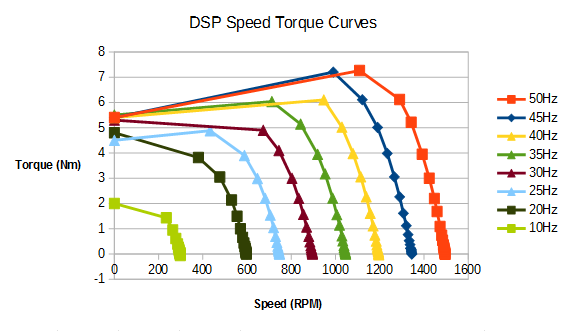
\includegraphics[scale=0.8]{DSP_pC_1}
		\caption{Results from the dynamometer for various frequencies}
		\label{fig:DSP_results}	
	\end{figure}
	\begin{figure}[H]
		\centering
		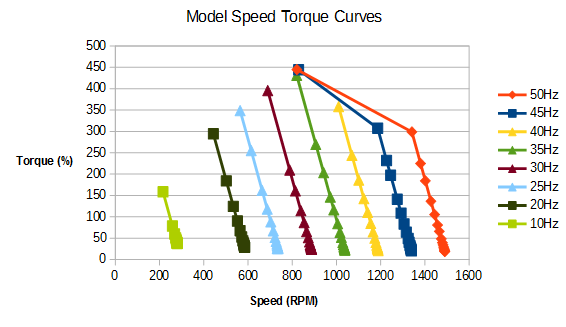
\includegraphics[scale=0.8]{Model_pC_1}
		\caption{Results from the motor drive panel for various frequencies}
		\label{fig:Model_results}
	\end{figure}
	
	\chapter{Analysis and Discussion}
	
	\section{Experimental vs Theory}
	
	\section{50Hz Low Slip Region}
	
	Figure 3.1 shows that in the 50 Hz data from the dynamometer, there is a linear trend in the low slip region. This region is from 1496 RPM to 1392 RPM, and is approximated by the linear equation shown in Equation \ref{eq:actual_approx}.
	\begin{align}
		T = -0.040\omega + 60.027
		\label{eq:actual_approx}
	\end{align}
	
	The theoretical curve is given by Equation \ref{eq:theoretical}.
	
	\begin{align}
	T = -0.033\omega + 49.435
	\label{eq:theoretical}
	\end{align}
	
	These curves can be seen in Figure \ref{fig:pC_3}.
	
	\begin{figure}[h]
		\centering
		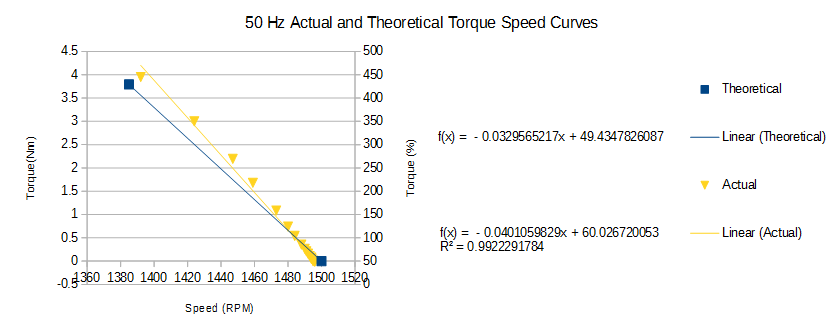
\includegraphics[width=\textwidth]{pC_3}
		\caption{Low slip region of 50 Hz data from dynamometer and theoretical curve from Part A}
		\label{fig:pC_3}
	\end{figure}
	
	These equations are quite similar, which indicates that the theoretical model of the low slip region provides an adequate approximation of the motor. 
	
	\section{Relationship Between Different Frequencies}
	
	The data collected from the dynamometer for various frequencies has been plotted in Figure \ref{fig:pC_4} below.
	
	\begin{figure}[H]
		\centering
		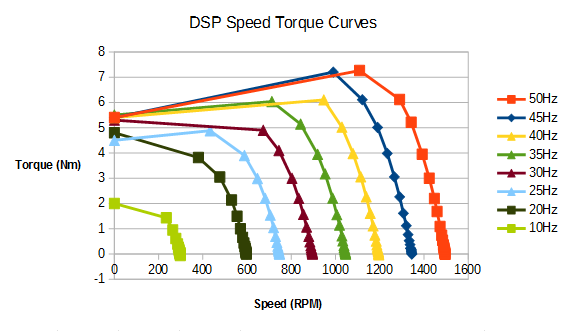
\includegraphics[scale=0.8]{DSP_pC_1}
		\caption{Results from the DSP for various frequencies}
		\label{fig:pC_4}	
	\end{figure}
	
	
	
	\section{Voltage and Speed Requirements to Drive Nominal Load at Set Speed}
	
	\chapter{Design Analysis}
	
	\chapter{Conclusions}
	
	\chapter{Recommendations}
	
	\chapter{References}
	
	\chapter{Appendices}
	
	
\end{document}          
